\documentclass[a4paper,12pt]{report}
\usepackage[utf8]{inputenc}
\usepackage[T1]{fontenc}
\usepackage{graphicx}
\usepackage{geometry}
\usepackage{setspace}
\usepackage{titling}
\usepackage{fancyhdr}
\usepackage{ifthen}
\usepackage{lastpage}
\usepackage[french]{babel}
\usepackage{amsmath} % Pour citation dans code block ? A tester si c'set bon ou non
\usepackage{xurl}  % Permet de casser les URL de manière améliorée
\usepackage[breaklinks]{hyperref}  % Permet de casser les liens URL
\usepackage{listings} % Importation du package pour le code source
\usepackage{xcolor}   % Importation du package pour la coloration syntaxique
\usepackage{float}
\usepackage{enumitem} % Pour sous-lister différements (* au lieu de -)

\usepackage[toc,nonumberlist]{glossaries}
\makeglossaries
\newglossaryentry{dynamique_vehicule}{
    name={dynamique de véhicule},
    plural={dynamique des véhicules},
    description={Ensemble des lois physiques qui régissent le mouvement, la stabilité et le comportement d’un véhicule}
}

\newglossaryentry{integration_numerique}{
    name={intégration numérique},
    description={Méthode permettant d’approximer la solution des équations différentielles dans les simulations en temps réel}
}

\newglossaryentry{euler_explicite}{
    name={méthode d'Euler},
    description={Technique d’intégration numérique simple utilisée pour mettre à jour l’état d’un système (vitesse, position, etc.)}
}

\newglossaryentry{derivee}{
    name={dérivée},
    description={Taux de variation instantané d'une fonction par rapport à une variable. Si \( f(x) \) est une fonction, sa dérivée \( f'(x) \) représente la pente de la tangente en \( x \) et s'exprime sous la forme \( \frac{d}{dx} f(x) \).}
}

\newglossaryentry{vitesseAngulaire}{
    name={vitesse angulaire},
    description={Taux de variation de l'angle de rotation d'un objet en fonction du temps. Elle est notée \( \omega \) et s'exprime en radians par seconde (\(\text{rad/s}\)). Elle est définie par \( \omega = \frac{d\theta}{dt} \), où \( \theta \) est l'angle de rotation.}
}

\newglossaryentry{equationDifferentielle}{
    name={équation différentielle},
    plural={équation différentielles},
    description={Équation reliant une fonction inconnue à ses dérivées. Elle permet de modéliser des phénomènes dynamiques en physique, en ingénierie et en mathématiques appliquées. Une équation différentielle ordinaire s'écrit sous la forme \( F(x, y, y', y'', \dots) = 0 \), tandis qu'une équation aux dérivées partielles fait intervenir des dérivées par rapport à plusieurs variables.}
}


\newglossaryentry{accelerationAngulaire}{
    name={accélération angulaire},
    description={Variation du vecteur \protect\gls{vitesseAngulaire} au cours du temps. Elle est notée \( \alpha \) et s'exprime en radians par seconde au carré (\(\text{rad/s}^2\)).}
}

\newglossaryentry{rotationAngulaire}{
    name={rotation angulaire},
    description={Mouvement de rotation d'un objet autour d'un axe. L'angle de rotation est généralement mesuré en radians et peut être décrit par la fonction \( \theta(t) \) représentant la position angulaire en fonction du temps.}
}


\newglossaryentry{modele_bicycle}{
    name={modèle bicycle},
    plural={modèle Bicycle},
    description={Modèle mathématique regroupant les roues avant et arrière en deux entités distinctes afin de simplifier la simulation de la dynamique du véhicule}
}

\newglossaryentry{angle_glissement}{
    name={angle de glissement},
    plural={angles de glissement},
    description={Angle formé entre la direction réelle d’un pneu et son orientation, déterminant la force latérale développée}
}

\newglossaryentry{sous_virage}{
    name={sous-virage},
    description={Comportement où le véhicule tourne moins que la trajectoire attendue, généralement dû à une perte d’adhérence à l’avant}
}

\newglossaryentry{survirage}{
    name={survirage},
    description={Comportement où le véhicule tourne plus que prévu, souvent lié à une perte d’adhérence à l’arrière}
}

\newglossaryentry{centre_gravite}{
    name={centre de gravité},
    description={Point de concentration de la masse d’un véhicule, influençant sa stabilité et la répartition des forces}
}

\newglossaryentry{essieu}{
    name={essieu},
    description={Composant reliant les roues d’un véhicule sur le même axe, dont la répartition du poids influe sur la dynamique}
}

\newglossaryentry{moment_inertie}{
    name={moment d'inertie},
    description={Mesure de la résistance d’un corps à un changement de rotation, calculée à partir de la masse et de la répartition des distances par rapport au centre de gravité}
}

\newglossaryentry{cyclesCPU}{
    name={cycles CPU},
    description={Unité de mesure représentant le temps nécessaire pour qu'un processeur exécute une instruction ou un ensemble d'instructions. Chaque cycle correspond à une impulsion d'horloge du processeur, et la performance d'un programme dépend souvent du nombre de cycles CPU consommés.}
}


\newglossaryentry{raideur_pneus}{
    name={raideur des pneus},
    description={Caractéristique des pneus qui détermine leur réponse aux forces appliquées. Voir aussi \gls{raideur_longitudinale} et \gls{raideur_laterale}}
}

\newglossaryentry{raideur_longitudinale}{
    name={Raideur longitudinale},
    plural={raideur longitudinale},
    description={Mesure de la réactivité des pneus aux forces de traction ou de freinage}
}

\newglossaryentry{raideur_laterale}{
    name={Raideur latérale},
    plural={raideur latérale},
    description={Mesure de la réponse des pneus aux forces générées lors des virages}
}

\newglossaryentry{glissement_dynamique}{
    name={Glissement dynamique},
    description={Évolution dans le temps du glissement d’un pneu par rapport à la surface de la route}
}

\newglossaryentry{saturation_forces_laterales}{
    name={Saturation non linéaire des forces latérales},
    description={Phénomène limitant la force latérale qu’un pneu peut générer une fois qu’un certain angle de glissement est dépassé}
}

\newglossaryentry{coefficient_adherence}{
    name={Coefficient d'adhérence},
    description={Paramètre définissant l’adhérence maximale d’un pneu sur la route, influençant les comportements de sous-virage et survirage}
}

\newglossaryentry{delta_temps}{
    name={delta de temps},
    description={Intervalle de temps entre deux itérations de la simulation, essentiel pour l’intégration numérique}
}

\newglossaryentry{gnuplot}{
    name={Gnuplot},
    plural={gnuplot},
    description={Outil de traçage graphique utilisé pour visualiser les résultats de la simulation (courbes de vitesse, trajectoire, etc.)}
}

\newglossaryentry{cpp}{
    name={C++},
    description={Langage de programmation orienté objet, utilisé pour le développement du simulateur}
}

\newglossaryentry{sfml}{
    name={SFML},
    description={\og Simple and Fast Multimedia Library \fg{}, Bibliothèque \gls{cpp} facilitant la création d’applications graphiques et multimédia}
}

\newglossaryentry{opengl}{
    name={OpenGL},
    description={API de rendu graphique 2D et 3D, utilisée par \gls{sfml} pour le rendu graphique}
}

\newglossaryentry{hud}{
    name={HUD},
    description={Système d’affichage superposé sur l’écran, utilisé ici pour présenter des informations telles que le compteur de \gls{fps} et les données de débogage}
}

\newglossaryentry{cmake}{
    name={CMake},
    plural={cmake},
    description={Outil de configuration et de gestion de compilation des projets \gls{cpp}}
}

\newglossaryentry{sprite}{
    name={sprite},
    description={Objet graphique représentant une image ou une animation dans un environnement 2D, utilisé pour afficher le véhicule et le circuit}
}

\newglossaryentry{std_deque}{
    name={std::deque},
    description={Structure de données de la \gls{stl} \gls{cpp} utilisée pour gérer une file de deltas de temps}
}

\newglossaryentry{std_vector}{
    name={std::vector},
    description={Conteneur dynamique de la \gls{stl} \gls{cpp} servant à stocker des données, par exemple, les points de la trajectoire prédictive}
}

\newglossaryentry{std_nth_element}{
    name={std::nth\_element},
    description={Algorithme de la \gls{stl} \gls{cpp} permettant d’obtenir efficacement l’élément médian dans un conteneur non trié}
}

\newglossaryentry{std_sort}{
    name={std::sort},
    description={Algorithme de tri de la \gls{stl} \gls{cpp} utilisé pour ordonner les éléments d’un conteneur}
}

\newglossaryentry{std_unordered_map}{
    name={std::unordered\_map},
    description={Structure de données de la \gls{stl} \gls{cpp} qui associe des clés à des valeurs, utilisée pour la gestion des ressources (textures, etc.)}
}

\newglossaryentry{sf_vertex_array}{
    name={sf::VertexArray},
    description={Classe de la \gls{sfml} permettant de représenter un ensemble de sommets, utilisée pour dessiner des formes complexes}
}

\newglossaryentry{deque}{
    name={deque},
    description={De l'anglais \og Double-ended queue \fg{}, structure de données permettant d’ajouter ou de retirer des éléments à chaque extrémité}
}

\newglossaryentry{std_unique_ptr}{
    name={std::unique\_ptr},
    description={Pointeur intelligent de la \gls{stl} \gls{cpp} assurant la gestion automatique de la mémoire pour des objets, par exemple, la police de caractères}
}

\newglossaryentry{stl}{
    name={bibliothèque standard},
    description={\og Standard Template Library \fg{}, bibliothèque standard de \gls{cpp} fournissant des conteneurs, algorithmes et itérateurs}
}

\newglossaryentry{git}{
    name={Git},
    description={Système de gestion de versions distribué, utilisé pour le suivi des modifications du code source}
}

\newglossaryentry{git_branches}{
    name={branches},
    description={Branches de développement dans \gls{git}, permettant de travailler sur différentes fonctionnalités ou corrections de bugs sans affecter la branche principale}
}

\newglossaryentry{stackoverflow}{
    name={Stack Overflow},
    description={Site de questions-réponses pour les développeurs, utilisé pour trouver des solutions à des problèmes techniques rencontrés lors du développement}
}

\newglossaryentry{arch-linux}{
    name={Arch Linux},
    description={Distribution Linux légère et rapide dont le concept est de rester la plus simple possible}
}

\newglossaryentry{ubuntu}{
    name={Ubuntu},
    description={Distribution Linux populaire, basée sur Debian, connue pour sa facilité d'utilisation et sa large communauté}
}

\newglossaryentry{pointer}{
    name={pointeur},
    description={Variable qui stocke l'adresse mémoire d'une autre variable, utilisée pour gérer la mémoire dynamique et les ressources}
}

\newglossaryentry{cpp_reference}{
    name={référence \gls{cpp}},
    description={Similaire à un \gls{pointer}, mais ne peut pas être modifiée pour pointer vers un autre objet après sa création.
    Elle est souvent utilisée pour passer des arguments à des fonctions sans les copier}
}

\newglossaryentry{boost}{
    name={Boost},
    description={Bibliothèque \gls{cpp} offrant des fonctionnalités supplémentaires, notamment pour la manipulation de flux et l'interfaçage avec d'autres outils}
}

\newglossaryentry{googletest}{
    name={Google Test},
    description={Framework de test unitaire pour \gls{cpp}, utilisé pour écrire et exécuter des tests automatisés}
}

\newglossaryentry{view}{
    name={vue},
    plural={vues},
    description={View, en anglais. Dans le contexte de l'interface graphique, cela fait référence à la manière dont les éléments sont affichés à l'utilisateur}
}

\newglossaryentry{multi_threading}{
    name={Multi-threading},
    description={Technique de programmation permettant l'exécution concurrente de plusieurs threads (unités d'exécution) au sein d'un même processus, améliorant ainsi la réactivité et la performance des applications}
}

\newglossaryentry{fps}{
    name={FPS},
    description={\og Frames Per Second \fg{}, mesure du nombre d'images affichées par seconde dans une animation ou un jeu vidéo, indiquant la fluidité de l'affichage}
}

\newglossaryentry{complexity}{
    name={complexité},
    description={Mesure de la quantité de ressources (temps, espace) nécessaires pour exécuter un algorithme ou une opération, souvent exprimée en fonction de la taille des données d'entrée}
}

\newglossaryentry{github}{
    name={GitHub},
    description={Plateforme de développement collaboratif basée sur \gls{git}, permettant de gérer des projets, de suivre les modifications et de collaborer avec d'autres développeurs}
}

\newglossaryentry{drracket} {
    name={DrRacket},
    description={Environnement de développement intégré (IDE) pour le langage de programmation Racket, utilisé principalement pour l'enseignement de l'informatique et le développement de logiciels}
}

\newglossaryentry{jruby} {
    name={JRuby},
    description={Implémentation du langage de programmation Ruby sur la machine virtuelle Java (JVM), permettant l'intégration avec les bibliothèques et outils Java}
}

\newglossaryentry{csharp} {
    name={C\#},
    description={Langage de programmation orienté objet développé par Microsoft, utilisé pour le développement d'applications sur la plateforme .NET}
}

\newglossaryentry{ruby} {
    name={Ruby},
    description={Langage de programmation interprété, orienté objet, connu pour sa simplicité et sa productivité, souvent utilisé pour le développement web}
}

\newglossaryentry{java} {
    name={Java},
    description={Langage de programmation orienté objet, conçu pour être portable et indépendant de la plateforme, largement utilisé pour le développement d'applications d'entreprise et mobiles}
}


% Définition du style pour le code Cpp
\lstdefinestyle{CStyle}{
    language=C++,
    basicstyle=\ttfamily\small,
    keywordstyle=\color{blue},
    commentstyle=\color{gray},
    stringstyle=\color{red},
    numbers=left,
    numberstyle=\tiny\color{gray},
    stepnumber=1,
    breaklines=true,
    frame=single,
    inputencoding=utf8,
    extendedchars=\true,
    literate={é}{{\'e}}1
             {è}{{\`e}}1
             {à}{{\`a}}1
             {ê}{{\^e}}1
             {ô}{{\^o}}1
             {ù}{{\`u}}1
}

\lstdefinestyle{BashStyle}{
    language=bash,
    basicstyle=\ttfamily\small,
    keywordstyle=\color{blue},
    commentstyle=\color{gray},
    stringstyle=\color{red},
    numbers=left,
    numberstyle=\tiny\color{gray},
    stepnumber=1,
    breaklines=true,
    frame=single,
    morekeywords={sudo,apt,echo,ls,cd,mkdir,rm,mv,cp,chmod,chown,grep,awk,sed,tar,zip,unzip,xxd,git,cmake,make,\&\&}
}



\def\UrlBreaks{\do\/\do-}

\renewcommand\thesection{\Roman{section}} % Numérotation des sections en chiffres romains
\renewcommand\thesubsection{\arabic{subsection}} % Numérotation des sous-sections en chiffres arabes
\renewcommand\thesubsubsection{\alph{subsubsection}} % Numérotation des sous-sous-sections en lettres minuscules
\setcounter{secnumdepth}{3} % Activer la numérotation jusqu'aux sous-sous-sections

% Pour gerer l'espace dans la table of contents
\usepackage{tocloft}
\renewcommand{\cftsecnumwidth}{2.3em}
\renewcommand{\cftsubsecnumwidth}{2.3em}

\hypersetup{
    colorlinks=true,
    linkcolor=black, % Couleur des liens internes (table des matières, etc.)
    urlcolor=blue, % Couleur des liens externes (URLs)
    citecolor=blue, % Couleur des liens de citation
    filecolor=blue % Couleur des liens vers des fichiers
}

\fancyhf{} % Efface les en-têtes et pieds de page par défaut
\pagestyle{fancy}
\renewcommand\headrulewidth{1pt}
\fancyhead[L]{Romain GALLAND | Quentin RADLO}
\fancyhead[R]{Université Marie \& Louis Pasteur}
\renewcommand\footrulewidth{1pt}
\fancyfoot[L]{ }
\fancyfoot[C]{Rapport de Projet - Simulateur de conduite\\
\textbf{Page \thepage/\pageref{LastPage}}}
\fancyfoot[R]{ }
\geometry{
    bindingoffset=1cm,  % Décalage pour la reliure
    left=2cm,
    right=2cm,
    top=2.5cm,
    bottom=2.5cm
}

\setlength{\headheight}{14.5pt}
\addtolength{\topmargin}{-2.5pt}

\begin{document}
    \begin{titlepage}

        \begin{center}
            \vspace{2cm}
            
\includegraphics[width=0.3\textwidth]{resources/university_logo}\par
        \end{center}



        \begin{center}
            \vspace{0.2cm}
            {\scshape \large{Rapport de projet} \par}
            Licence 3 Informatique - UFR Sciences et Techniques
            \vspace{0.4cm}
            \hrule
            \vspace{0.4cm}
            {\huge\bfseries Simulateur de conduite \par}
            \vspace{0.4cm}
            \hrule
            \vspace{1cm}
            {\large\bfseries Décembre 2024 - Mars 2025 \par}
            Romain GALLAND - Quentin RADLO
            %\vspace*{1.5cm}
            % Image d'illustration
            % \vspace*{1.5cm}
            \vspace{1cm}
            \begin{center}
                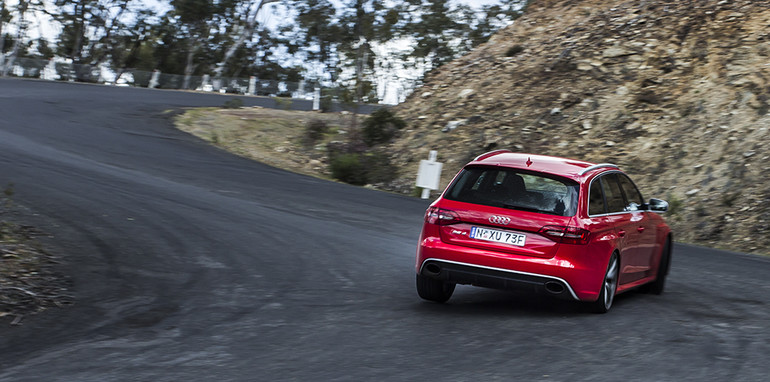
\includegraphics[width=0.8\textwidth]{resources/illustration}
            \end{center}


            % Informations supplémentaires
            \vspace{1cm}
            {\bfseries Sous la supervision de:} Jean-Michel Hufflen \\


        \end{center}
    \end{titlepage}


    \newpage
    \section*{Remerciements}
    - Un remerciement particulier est adressé à M. Hufflen pour la direction et la pédagogie qu'il nous a apporté lors de la réalisation de notre projet.

    % Page dédiée à la table des matières
    \newpage
    \tableofcontents

    \usepackage{glossaries}\section{Sujet du projet}\label{sec:sujet-du-projet}
Avant tout, il est important de noter que, chaque première utilisation d'un terme présent dans le glossaire sera suivi d'un astérisque, de la sorte : exemple^{*}.
\subsection{Le sujet}\label{subsec:le-sujet}
Le sujet originel nous laissait une assez grande liberté quant à l'orientation de notre projet.
L'idée globale consistait en la réalisation graphique d'un mini-simulateur de conduite, avec des ordres de conduite (démarrage, arrêt, accélération et décélération) donnés par la frappe du clavier.
L'utilisateur devait pouvoir observer son véhicule ainsi que le circuit avec une vue du dessus ou la vision du conducteur à travers le pare-brise.
Il était aussi proposé de pouvoir \og corser\fg{} le jeu en programmant des événements aléatoires.

Pour réaliser ce projet, plusieurs langages de programmation nous étaient proposés :
\begin{itemize}
    \item \textbf{\gls{drracket}}, avec des compléments pour nous aider sur la partie graphique.
    \item \textbf{\gls{jruby}}, avec pour idée d'implémenter la logique du programme en \gls{ruby} et la partie graphique avec des bibliothèques de \gls{java}.
    \item \textbf{\gls{csharp}} ou \textbf{\gls{cpp}} avec les bibliothèques graphiques adéquates.
\end{itemize}


\subsection{Notre interprétation du sujet}\label{subsec:notre-interpretation-du-sujet-/-objectif-du-sujet}
Après réflexion et discussion avec notre tuteur, nous avons décidé de partir vers une orientation de didacticiel plutôt qu'une \og orientation de \("\)jeu\("\) \fg{}.
L'idée était d'implémenter un modèle de \gls{dynamique_vehicule}\textsuperscript{*} se rapprochant de la réalité.
Avec un tel modèle, nous pourrions donc visualiser des comportements de perte d'adhérence sur route, ainsi que les phénomènes de \gls{survirage} et \gls{sous_virage}.
Un tel simulateur permettrait ainsi à l'utilisateur d'expérimenter / se familiariser avec les comportements du véhicule.
Pour le langage de programmation, nous avons décidé de nous orienter vers le langage \gls{cpp}, car il nous était plus familier que les autres langages proposés, et nous avons utilisé \gls{sfml} en tant que bibliothèque graphique.
Ensuite, nous avons donc commencé l'implémentation de notre simulateur, il s'est décomposé en deux grandes parties, l'implémentation de la physique et la création de l'interface graphique.
Nous allons commencer par vous présenter la partie physique de notre projet.

\newpage
    \subsection{Introduction}\label{subsec:introduction}
Pour représenter la relation entre un véhicule et la route d'une manière se rapprochant de la réalité, nous avons donc dû implémenter des phénomènes physiques venant des sciences de l'ingénieur. De plus, comme l'étude et la représentation d'un système  de dynamique de véhicule est une tâche plutôt difficile, nous avons décidé de procéder de manière itérative. Tout d'abord, le but était d'avoir une implémentation très basique d'un système de dynamique,  puis une fois celui-ci fonctionnel, d'itérer ce système pour intégrer des phénomènes plus délicats à implémenter, puis d'encore itérer sur ce système, etc.
Ceci nous a mené à un plan en 5 étapes.
Premièrement, implémenter les lois de Newton pour la dynamique du véhicule, puis implémenter un modèle bicycle simplifié, pour ensuite pouvoir représenter les forces sur les pneus et modéliser les glissements, et finalement pouvoir simuler les limites du pneumatique.
Nous allons maintenant vous détailler les principes physiques et l'implémentation que nous avons fournis pour chacune de ces étapes :

\subsection{Implémentation des lois de Newton pour la dynamique du véhicule}\label{subsec:implementation-des-lois-de-newton-pour-la-dynamique-du-vehicule}

Comme base de notre projet, nous avons donc commencé par implémenter la première Loi de Newton qui est le principe d'inertie, il stipule que tout corps conservera son état de repos ou de mouvement rectiligne uniforme en ligne droite dans lequel il se trouve, à moins qu'une force ne soit appliquée sur ce corps. Ainsi, un système ou corps quelconque ne peut pas se déplacer à moins qu'une force ne lui soit appliquée. Et c'est pareil pour qu'un système passe d'un état de mouvement à un état arrêté.
Dans notre implémentation, cette loi est traduite par le fait que si aucune force n'agit sur le véhicule, alors ses vitesses vont rester nulles (ou constantes si le véhicule est initialisé avec une vitesse).
Pourquoi et comment avons-nous implémenté cette loi ?
Rappelons d'abord que l'équation fondamentale de la dynamique est donnée par :
$$F = m \ .\  a$$
Avec :
\begin{itemize}
    \item $F$ la force appliquée sur le corps,
    \item $m$ la masse du corps,
    \item $a$ l'accélération résultante.
\end{itemize}

Dans notre code, nous avons appliqué cette relation en calculant les accélérations $a_x$ et $a_y$ du véhicule à partir des forces appliquées :


\begin{lstlisting}[style=CStyle,label={lst:void_computeTranslation}]
void computeTranslation(const double Fx, const double Fy, double& ax, double& ay) {
    ax = Fx / m;
    ay = Fy / m;
}
\end{lstlisting}

Ici si $F_x = 0$ et $F_y = 0$, alors $a_x$ et $a_y$, s'annulent, ce qui signifie que les vitesses restent constantes conformément au principe d'inertie.
Cependant, dès qu'on applique une force sur un objet, on génère une accélération. Cette accélération va alors modifier la vitesse de l'objet, et, comme la position est liée à la vitesse de l'objet, alors, elle évoluera dans le temps. Ce processus est décrit par des équations différentielles. Dans notre cas, nous aurons :
$$\frac{d v_x}{dt} = a_x, \quad \frac{d v_y}{dt} = a_y, \quad \frac{d r}{dt} = r_{\dot{}}$$
où $v_x$ et $v_y$ représentent les composantes de la vitesse et $r$ le lacet, l'orientation, du véhicule.

Cependant, comme notre simulateur est en temps réel, résoudre ces équations à chaque itération demanderait de nombreux cycles CPU, alors pour préserver leur usage, nous utilisons une méthode numérique, celle qui est la plus simple et efficace : la \textbf{méthode d'Euler explicite}.

Cette méthode repose sur le fait que la dérivée d'une variable $x$ notée $\dot{x}$ reste constante sur un petit intervalle de temps $dt$. Donc, on peut approximer son évolution par :
$$x(t+dt) \approx x(t) + \dot{x}(t) \times dt$$
Dans la première implémentation de notre simulateur, nous utilisons donc cette formule pour mettre à jour les vitesses et l'orientation de la voiture :
\\
\begin{itemize}
    \item \textbf{Pour la vitesse sur l'axe $x$ :}
    $$v_x(t+dt) = v_x(t)+a_x(t)\times(dt)$$
    \item \textbf{Pour la vitesse sur l'axe $y$ :}
    $$v_y(t+dt) = v_y(t)+a_y(t)\times(dt)$$
    \item \textbf{Pour l'orientation $r$ :}
    $$r(t+dt) = r(t)+\dot{r}(t)\times(dt)$$
\end{itemize}
Ici, on utilise $a_x(t)$, car c'est la dérivée de $v_x(t)$ par rapport au temps. C'est la même chose pour $a_y(t)$ qui résulte de $a_y(t)$. Ensuite, pour trouver $\dot{r}(t)$, qui est l'accélération angulaire, on applique la loi de la dynamique de rotation angulaire qui est la suivante :
$$I\dot{r}(t) = \texttt{torque}$$
où $I$ est le moment d'inertie de l'objet. En isolant $\dot{r}(t)$, on obtient :
$$\dot{r}(t)= {\frac{\texttt{torque}}{}}$$
Nous calculons cette valeur via un appel à la fonction \texttt{computeYawAcceleration(torque);} où cette relation est implémentée.

Grâce à cela, l'état de notre véhicule est mis à jour en obtenant une approximation de la solution des équations différentielles, plutôt que de les résoudre, ce qui prendrait plus de temps de calcul.
Cependant, la précision de la méthode d'Euler dépend forcément de la taille du pas qu'on lui donne ($dt$), et c'est la même chose pour des systèmes plus complexes. Dans ces cas-ci, cette méthode produira alors des erreurs significatives et la simulation deviendra instable. C'est pourquoi, plus tard dans l'implémentation de notre physique, nous avons choisi d'implémenter une méthode plus fiable dans ces cas-ci.

Ensuite, pour valider le bon fonctionnement des principes physiques que nous avons décrit et implémenté, nous avons réalisé une simulation de 10 secondes (avec un pas de 0,1 s), et avons utilisé \textbf{Gnuplot} pour visualiser les résultats obtenus et observer si le résultat obtenu est celui attendu. Voici la manière dont nous initialisons notre objet voiture, et indiquons la démarche à suivre pour avoir une simulation sur 10 secondes :
\begin{lstlisting}[style=CStyle,label={lst:void_simulation_etape1}]
void simulation_etape1() {
    // Initialisation du vehicule (mass=1700 kg, dist_cog_front_axle=1.5 m, dist_cog_rear_axle=1.5 m)
    OldVehicle myVehicle(1700.0, 1.5, 1.5);

    // Parametres de simulation
    double Fx = 500.0;       // Force longitudinale (N)
    double Fy = 200.0;       // Force laterale (N)
    double torque = -150.0;  // Moment de lacet (Nm)
    double dt = 0.1;         // Pas de temps (s)
    int steps = 10000;       // Simulation sur 10 secondes

    // Vecteurs pour stocker les donnees : paire (temps, valeur)
    std::vector<std::pair<double, double>>vx_data, vy_data, r_data;

    // Simulation : enregistrement des etats a chaque pas de temps
    for (int i = 0; i <= steps; ++i) {
        vx_data.push_back({t, myVehicle.vx});
        vy_data.push_back({t, myVehicle.vy});
        r_data.push_back({t, myVehicle.lacet
        myVehicle.update(dt, Fx, Fy, torque);
    }
    // ... Plot des donnees stockees dans les vecteurs avec Gnuplot

}
\end{lstlisting}

{\LARGE Question => Doit-on ajouter la partie code Gnuplot à la figure précédente ?}

Les graphiques donnés par notre implémentation donnent alors :

\begin{center}
    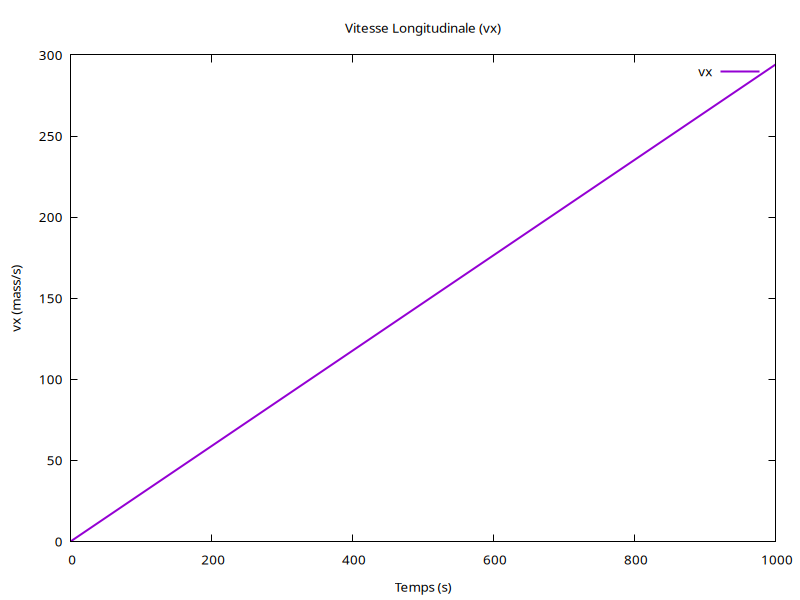
\includegraphics[width=0.70\linewidth]{Plots_Etape1/vx}
    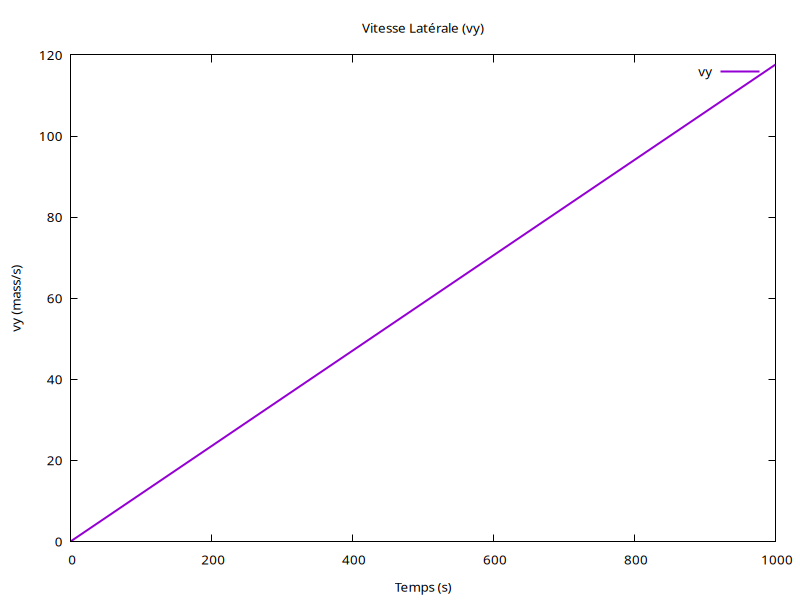
\includegraphics[width=0.70\linewidth]{Plots_Etape1/vy}
    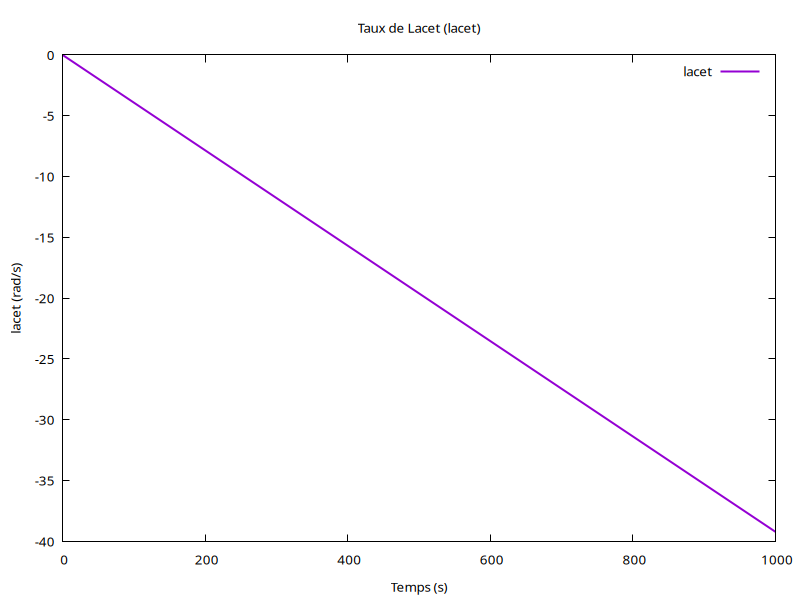
\includegraphics[width=0.70\linewidth]{Plots_Etape1/lacet}
\end{center}



\begin{itemize}
    \item \textbf{Graphique de la vitesse longitudinale ($vx$)} : Sur ce premier graphique, on observe bien que l'évolution de la vitesse sur l'axe $y$, se traduit par l'application de la force longitudinale ($ F = m \cdot a $). Et nous avons donc une accélération constante, ce qui mène à une augmentation linéaire de $vx$ au fil du temps.

    \item \textbf{Graphique de la vitesse latérale ($vy$)} : De même, le graphique représentant $vy$ permet d'observer l'effet de la force latérale appliquée.

    \item \textbf{Graphique du taux de lacet ({$\texttt{lacet}$})} : Et dernièrement, ce graphique-ci nous permet de voir l'évolution de l'orientation du véhicule. Grâce à la loi de la dynamique de rotation ($I\dot{r} = \texttt{torque}$), nous constatons que l'accélération angulaire est directement proportionnelle au couple appliqué, ce qui se traduit par une variation linéaire de $\texttt{lacet}$ au fil du temps.
\end{itemize}

\subsection{Implémentation du modèle Bicycle simplifié}
Après avoir implémenté ces phénomènes physiques de base, nous devions rajouter une façon de pouvoir contrôler notre véhicule de manière réaliste. C'est pourquoi nous avons choisi d'implémenter le modèle Bicycle simplifié. C'est un modèle couramment utilisé en dynamique des véhicules, plutôt que de traiter séparément les quatre roues d'un véhicule, il regroupe les roues avant en une seule roue, et fait de même pour les roues arrière. En procédant de cette façon, nous pouvons capturer les comportements dynamiques des pneus d'un véhicule tout en réduisant la complexité des équations utilisées. Comme le but de cette partie était de pouvoir calculer la trajectoire d'un véhicule, nous avons utilisé le modèle bicycle pour trouver l'angle de glissement des pneus, ainsi que pour trouver les forces appliquées sur ceux-ci, pour pouvoir modéliser la trajectoire.
Mais qu'est-ce que l'\textbf{angle de glissement} ? L'angle de glissement est l'angle formé entre la direction réelle d'un pneu et l'orientation de la roue. Il est induit par les forces latérales lors d'un virage. Plus cet angle est grand, plus les forces latérales appliquées sur le pneu sont grandes. Chaque pneu a, en fonction de son revêtement et de la condition de la route sur laquelle il se trouve, une limite d'adhérence au-delà de laquelle il ne peut plus maintenir un contact optimal avec la route. Alors le pneu perd son efficacité et commence à déraper. Cet angle a une grande importance dans la dynamique des véhicules, car il influence leur stabilité et
leur comportement en virage.
C'est en implémentant cette limite, plus tard dans notre modèle, que nous avons pu simuler le comportement de sous-virage et de survirage.

\newpage{}
    \section{L'implémentation de l'interface graphique}\label{sec:l'implementation-de-l-interface-graphique}
\subsection{Bibliothèques utilisées (SMFL)}\label{subsec:sfml}
\gls{sfml} (\textit{Simple and Fast Multimedia Library}) est une bibliothèque \gls{cpp} qui permet de créer des applications multimédia.
Elle est particulièrement adaptée pour le développement de jeux vidéo et d'applications graphiques.
Elle fournit des fonctionnalités pour la gestion des fenêtres, le rendu graphique, la gestion des événements, le son et la communication réseau.
En interne, elle s'appuie sur \gls{opengl}, une bibliothèque plus bas niveau, ce qui permet d'obtenir d'excellentes performances graphiques tout en restant simple d'utilisation.

\gls{sfml} a été choisie pour plusieurs raisons :
\begin{itemize}
    \item \textbf{simplicité d'utilisation} : elle permet de se concentrer sur la logique applicative plutôt que sur des détails techniques complexes,
    \item \textbf{documentation et communauté} : sa documentation\cite{documentationSFML} est complète et une large communauté offre de nombreux exemples et ressources,
    \item \textbf{multiplateforme} : la compatibilité avec Windows, Linux et macOS permet de développer l'application sans penser à la portabilité.
\end{itemize}

\subsection{Architecture de l'interface graphique}\label{subsec:architecture-de-l-interface-graphique}
\subsubsection{Organisation modulaire du code}\label{subsubsec:organisation-modulaire-du-code}
Afin d'assurer une bonne lisibilité et une maintenance du code plus simple, l'interface graphique a été développée de manière modulaire.
Chaque fonctionnalité est séparée dans une classe spécifique.
Par exemple, la gestion du véhicule, du circuit et des indicateurs de débogage est confiée à des modules distincts.
Cette organisation rend également l'intégration de nouvelles fonctionnalités plus aisée sans nécessiter de modifications majeures dans la structure existante.

Le diagramme de classe UML de l'interface graphique est disponible en page suivante (fig.~\ref{fig:uml_diagram}).

\begin{figure}[H]
    \centering
    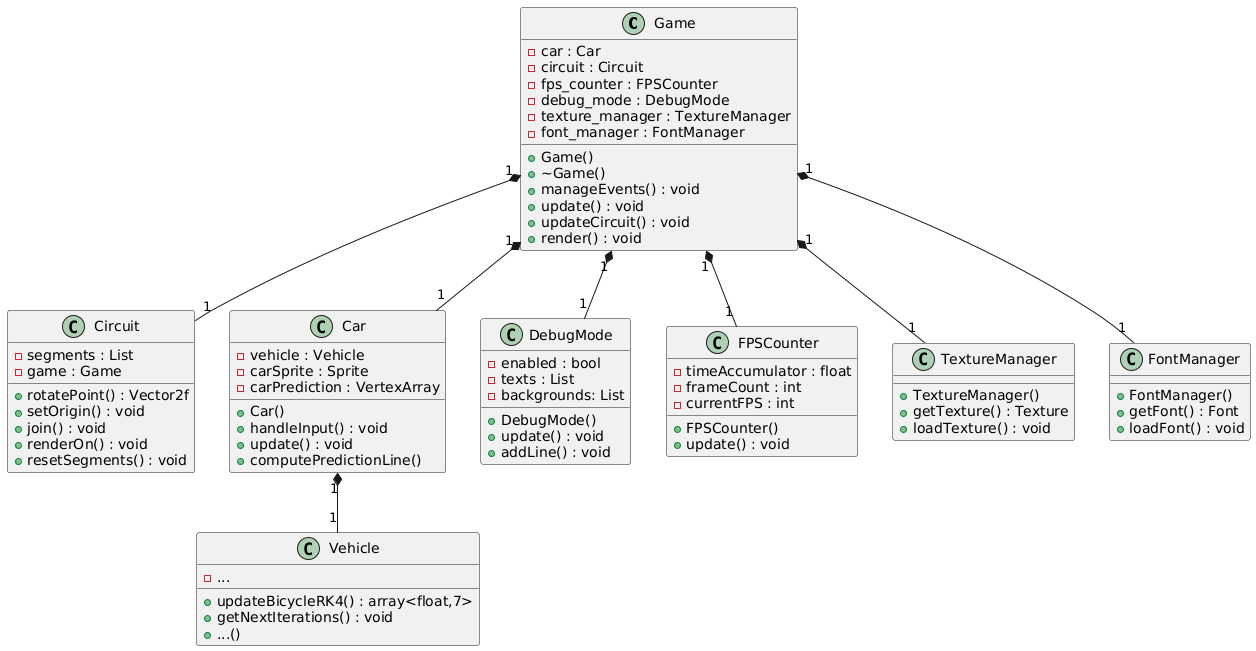
\includegraphics[width=0.7\textwidth]{resources/classdiagram}
    \caption{Diagramme de classe UML de l'interface graphique}
    \label{fig:uml_diagram}
\end{figure}

\subsubsection{Présentation des classes principales}\label{subsubsec:presentation-des-classes-principales}
Plusieurs classes essentielles interagissent pour constituer une interface graphique à la fois cohérente et fluide.

\paragraph[Game]{La classe \textbf{Game}}\label{par:class_game}
La classe \textbf{Game} constitue le noyau central du projet, orchestrant l'ensemble de l'application.
Elle se charge notamment d'initialiser la fenêtre \gls{sfml}, de configurer les différentes \glspl{view}\textsuperscript{*} (notamment la \texttt{Game \glslink{view}{View}} et la \texttt{\gls{hud} \glslink{view}{View}}), de gérer le cycle de vie de la simulation (mise à jour, gestion des événements et rendu) et de coordonner les interactions entre les divers modules.

Elle contient 3 fonctions principales :
\begin{lstlisting}[style=CStyle, label={lst:game_class}]
    void update();
    void render() const;
    void manageEvents();
\end{lstlisting}
Chaque méthode est appelée une fois par itération de la boucle principale de l'application et donc une fois par image générée.
Voici leurs rôles respectifs :
\begin{itemize}
    \item \texttt{update()}, met à jour l'état de l'application en fonction du temps écoulé et des événements utilisateurs.
    \item \texttt{render()}, effectue le rendu graphique de la scène actuelle.
    \item \texttt{manageEvents()}, gère les événements à l'intérieur de l'application (clavier, souris), elle est appelée dans la méthode \texttt{update()}.
\end{itemize}

\paragraph[Circuit]{La classe \textbf{Circuit}}
Elle représente, comme son nom l'indique, un circuit de conduite.
Elle est composée de différents segments de routes (comme une petite ligne droite, un petit virage, un grand virage, \dots).
Chaque segment est une portion de route qui peut être droite ou courbe, et la classe gère la connexion entre ces segments pour former une impression de circuit continue au niveau de l'affichage graphique. \\
Son fonctionnement interne permet, de l'extérieur de la classe, de simplifier la création de la route.
Il suffit de rajouter des segments de route dans le circuit en précisant l'angle à donner à la texture et s'il faut lui appliquer un effet mirroir, et la classe se charge de les relier entre eux.

L'extrait de code suivant permet de réaliser ce bout de circuit (fig.~\ref{fig:example_circuit_1}) :
\begin{lstlisting}[style=CStyle, label={lst:code_circuit}]
Circuit circuit;
circuit.setOrigin(ResourceType::Value::SEGMENT_SMALL_STRAIGHT);
circuit.join(ResourceType::Value::SEGMENT_S_TURN);
circuit.join(ResourceType::Value::SEGMENT_MEDIUM_TURN);
circuit.join(ResourceType::Value::SEGMENT_LARGE_TURN, 90);
circuit.join(ResourceType::Value::SEGMENT_U_TURN, 180);
circuit.join(ResourceType::Value::SEGMENT_U_TURN, 0, false, true);
circuit.join(ResourceType::Value::SEGMENT_LONG_STRAIGHT, 180);
\end{lstlisting}

\begin{figure}[h]
    \centering
    
\includegraphics[width=0.5\textwidth]{resources/example_circuit_1}
    \caption{Exemple de circuit pouvant être généré grâce à la classe Circuit}
    \label{fig:example_circuit_1}
\end{figure}

\paragraph[Car]{La classe \textbf{Car}}
Cette classe encapsule la classe \texttt{Vehicle} (voir section \ref{sec:l'implementation-de-la-physique-/-modelisation-d'un-systeme-de-dynamique-de-vehicule}).
L'interaction entre les deux classes \texttt{Car} et \texttt{Vehicle} est présentée au paragraphe~\ref{subsubsec:interactions-entre-l-interface-graphique-et-la-partie-physique}.
Elle calcule la ligne de prédiction de la trajectoire du véhicule et gère l'affichage du véhicule.

Lors du développement de la ligne de prédiction de trajectoire, nous avons rencontré un problème.
Le calcul prend en paramètre un \gls{delta_temps} (\texttt{dt}) qui correspond au temps entre la dernière image et l'image actuelle.
Ce \gls{delta_temps} est très volatile et peut varier du simple au double entre deux images, ce qui cause de grosses différences de longueur de la ligne de prédiction et provoque une impression de scintillement.

Pour résoudre ce problème, nous avons décidé de récupérer le \gls{delta_temps} médian sur les 1000 dernières images.

\begin{lstlisting}[style=CStyle, label={lst:code_dequeue_dt}]
std::deque<float> dtBuffer;
const size_t max_dt_buffer_size = 1000;
float updateAndGetMedian(const float dt) {
    dtBuffer.push_back(dt);
    if (dtBuffer.size() > max_dt_buffer_size) {
        dtBuffer.pop_front();
    }
    std::vector tmp(dtBuffer.begin(), dtBuffer.end());
    const auto mid = tmp.begin() + tmp.size() / 2;
    std::nth_element(tmp.begin(), mid, tmp.end());
    return *mid.base();
}
\end{lstlisting}

La \gls{complexity} de la méthode \texttt{updateAndGetMedian(const float dt)} est en \( O(n) \).
Voici le détail du calcul :
\begin{itemize}
    \item \texttt{push\_back(dt)} : \( O(1) \)\cite{cpp_reference_push_back} pour ajouter un élément à la fin de la \texttt{\gls{std_deque}}.
    \item \texttt{pop\_front()} : \( O(1) \)\cite{cpp_reference_pop_front} pour retirer le premier élément de la \texttt{\gls{std_deque}}.
    \item \texttt{\gls{std_vector} tmp(dtBuffer.begin(), dtBuffer.end())} : \( O(n) \)\cite{cpp_reference_vector} pour copier la \texttt{\gls{std_deque}} dans un conteneur du type \texttt{\gls{std_vector}}.
    \item \texttt{\gls{std_nth_element}(tmp.begin(), mid, tmp.end())} : \( O(n) \)\cite{cpp_reference_std_nth_element} pour trier le conteneur jusqu'à l'élément médian.
\end{itemize}

Nous avons utilisé la fonction de la \gls{stl} \texttt{\gls{std_nth_element}()}\cite{cpp_reference_std_nth_element} car elle permet de ne pas trier l'ensemble du conteneur tout en plaçant l'élément médian à la bonne position dans le \texttt{\gls{std_vector}}\cite{cpp_reference_vector}.
Au départ, nous avions choisi la fonction \texttt{\gls{std_sort}()}, qui trie un conteneur complet, mais la \gls{complexity} de la méthode aurait été en \( O(n \log n) \)\cite{cpp_reference_std_sort}, ce qui est moins optimal étant donné que la ligne de prédiction est recalculée à chaque image.


\subsubsection{Les ressources}\label{subsubsec:gestion-des-ressources}
\paragraph{Type de ressources}
Dans le projet, nous avons principalement deux types de ressources :
\begin{itemize}
    \item les \textbf{textures} : utilisées pour le rendu graphique des segments de route et du véhicule.
    \item les \textbf{olices de caractères} : utilisées pour le rendu du texte dans l'interface graphique.
\end{itemize}

\paragraph{Les textures}
Au sein de la librairie \gls{sfml}, une image est représentée avec une classe \texttt{sf::Texture}\cite{sfml_sf_texture} qui contient la représentation en mémoire de ses pixels.
Chaque texture (ou image) correspond à une entrée dans une enum \texttt{ResourceType::Value} qui permet de l'identifier de manière unique, cela concerne les segments de route ainsi que l'image de la voiture.
Cette enum est définie dans le fichier \texttt{resource\_type.h} et contient les valeurs suivantes :
\begin{itemize}
    \item \texttt{SEGMENT\_SMALL\_STRAIGHT} : une petite ligne droite.
    \item \texttt{SEGMENT\_LONG\_STRAIGHT} : une grande ligne droite.
    \item \texttt{SEGMENT\_SMALL\_TURN} : un virage moyen.
    \item \texttt{SEGMENT\_MEDIUM\_TURN} : un virage moyen.
    \item \texttt{SEGMENT\_LARGE\_TURN} : un virage large.
    \item \texttt{SEGMENT\_S\_TURN} : un virage en \texttt{S} (plus communément appelé une chicane)
    \item \texttt{SEGMENT\_U\_TURN} : un virage en \texttt{U}\@.
    \item \texttt{CAR} : la voiture.
\end{itemize}

\paragraph{La police d'écriture}
La police d'écriture utilisée dans le projet est la \textit{DejaVu Sans Mono}.
Pour une portabilité maximale de notre code, nous avons décidé de l'inclure directement dans le binaire de l'application.

Pour cela, nous avons généré un fichier \gls{cpp} contenant les données binaires de la police \textit{DejaVu Sans Mono} en utilisant la commande Bash suivante sous Linux:
\begin{lstlisting}[style=BashStyle,label={lst:generation_dejavusansmonottf_h}]
xxd -i DejaVuSansMono.ttf > dejavu_sans_mono_ttf.cpp
\end{lstlisting}
Cette commande (\texttt{\gls{xxd}}) convertit le fichier binaire de la police en un tableau d'octets de style C que nous pouvons inclure directement dans notre projet.
Le fichier généré contient deux éléments :
\begin{itemize}
    \item Un tableau d'octets contenant les données binaires de la police.
    \item La taille de ce tableau.
\end{itemize}

Cette solution, trouvée sur le site \gls{stackoverflow}\cite{stackoverflow_embed_font}, nous permet d'intégrer la police directement dans le fichier binaire de l'application, assurant ainsi une portabilité maximale.
Cette fonctionnalité est rendue possible grâce à la bibliothèque \gls{sfml} qui permet de charger une police à partir d'un tableau d'octets \textit{via} la fonction suivante :

\begin{lstlisting}[style=CStyle,label={lst:load_from_memory}]
bool Font::loadFromMemory(const void* data, std::size_t sizeInBytes);
\end{lstlisting}

Cette fonction prend en paramètre un pointeur vers le tableau contenant les données binaires de la police et la taille de ce tableau.
Il est important de noter que le tableau attendu est de type \gls{cstyle_array}, c'est-à-dire qu'il s'agit d'un simple bloc de mémoire brut, et non d'un objet \gls{cpp} encapsulé.

\paragraph{Gestionnaire de ressources}
Nous avons fait le choix de séparer la gestion de ces deux types de ressources en deux classes différentes étant donné leurs utilisations différentes.

La classe \texttt{TextureManager} gère le chargement des images dans la mémoire de l'application.
Lorsque l'on a besoin d'utiliser une instance de la classe \texttt{sf::Texture}\cite{sfml_sf_texture}, on fait appel à la méthode \texttt{TextureManager::getTexture()} qui prend en paramètre un \texttt{ResourceType::Value} et renvoie une \gls{cpp_reference} vers la texture correspondante.
Deux cas sont possibles :
\begin{itemize}
    \item La texture n'a jamais été demandée depuis le début de l'exécution, elle est donc chargée depuis le disque dur et stockée dans un conteneur de la \gls{stl}, une \texttt{\gls{std_unordered_map}<ResourceType::Value, sf::Texture>}\cite{cpp_reference_std_unordered_map}.
    \item La texture a déjà été chargée, une \gls{cpp_reference} vers l'instance de la classe \texttt{sf::Texture}\cite{sfml_sf_texture} correspondante est récupérée puis renvoyée.
    Ici, on utilise une \gls{cpp_reference} et non une copie, car aucun traitement n'est fait directement sur l'objet en mémoire.
\end{itemize}
Ce système permet de ne charger qu'une seule fois une texture et de la réutiliser à chaque fois qu'elle est demandée, ce qui limite grandement l'utilisation de la mémoire.

Pour ce qui est des polices de caractères, la classe \texttt{FontManager} fonctionne de manière similaire, mais nous n'utilisons qu'une seule police de caractères pour l'ensemble de l'application.
Lors de la création de l'objet, la police est chargée depuis le disque dur et stockée dans la mémoire dites \og \gls{heap} \fg{}.

Le seul attribut de la classe est un \gls{pointer} \gls{cpp} (du type \texttt{\gls{std_unique_ptr}}\cite{cpp_reference_std_unique_ptr} de la \gls{stl}) qui pointe vers l'instance de la classe \texttt{sf::Font} contenant la police de caractères.

\paragraph{Connexion des segments de routes}
En interne, la texture d'un segment de route est représentée par une structure \texttt{RoadTexture} définie comme suit :

\begin{lstlisting}[style=CStyle,label={lst:struct_roadtexture}]
struct RoadTexture {
    const sf::Texture *texture = nullptr;
    sf::Sprite sprite;
    sf::Vector2f point1;
    sf::Vector2f point2;
};
\end{lstlisting}

Elle contient 4 éléments :
\begin{itemize}
    \item \texttt{texture} : Un \gls{pointer} vers la texture de la route chargée par le \texttt{TextureManager}.
    \item \texttt{sprite} : Le \textit{\gls{sprite}} associé à la texture, utilisé pour le rendu.
    \item \texttt{point1} et \texttt{point2} : Deux positions relatives à la texture représentant les points de connexion entre deux segments de route du type \texttt{sf::Vector2f}, objet venant de la bibliothèque \gls{sfml} représentant un point, et donc deux coordonnées.
\end{itemize}

Lorsque l'on ajoute un nouveau segment \textit{via} la méthode \texttt{join()}, le processus se déroule comme suit :

\begin{enumerate}
    \item \textbf{Récupération du segment précédent :} % TODO modif cmplt
    On commence par récupérer le dernier segment inscrit dans le circuit (\textit{via} \texttt{segments.back()}).
    Ce segment précédent fournit la position finale (stockée dans l'attribut \texttt{realPoint2} de la structure \texttt{RoadSegment}) qui sera utilisée comme point de départ pour le nouveau segment.

    \item \textbf{Génération et configuration de la texture :}
    À l'aide de la méthode \\\texttt{generate\_road\_texture()}, la texture destinée au nouveau segment est créée \textit{via} le gestionnaire de textures, en prenant en compte les éventuelles opérations de mirroring (horizontal et/ou vertical).
    Ensuite, la texture, représentée par son \gls{sprite}, est redimensionnée selon le facteur de zoom actuel (obtenu grâce à la méthode \texttt{game->getZoomFactor()} de la classe \texttt{Game}, voir~\ref{par:class_game}) afin d'assurer une cohérence visuelle optimale.

    \item \textbf{Alignement du nouveau segment :}
    Pour garantir la continuité du circuit, l'origine du \gls{sprite} du nouveau segment est assignée au point de connexion initial (grâce à l'attribut \texttt{road\_texture.point1}).
    Ensuite, le \gls{sprite} est positionné précisément à l'endroit où se termine le segment précédent (grâce à l'attribut \texttt{fromPoint2} de ce segment), assurant ainsi que le nouveau segment débute exactement là où le précédent s'est terminé.

    \item \textbf{Calcul du point de raccord final avec rotation :}
    Afin de déterminer la position finale du nouveau segment, un décalage est calculé à partir de sa position initiale, selon les étapes suivantes :
    \begin{itemize}
        \item On commence par récupérer la position globale du \textit{\gls{sprite}} grâce à la méthode \texttt{spr->getGlobalBounds().getPosition()}.
        \item Ce point est ensuite ajusté en y ajoutant la valeur de l'attribut \\\texttt{road\_texture.point2} (après application du zoom), permettant ainsi d'estimer la position finale du segment en l'absence de rotation.
        \item Enfin, la méthode \texttt{rotatePoint()} est utilisée pour faire pivoter ce point autour du point de raccord initial selon l'angle spécifié.
        Le résultat obtenu, désigné par la variable locale \texttt{rotatedPoint}, définit à la fois l'orientation et la position finale du segment après rotation.
    \end{itemize}

    \item \textbf{Application de la rotation et ajout du segment :}
    Une fois le point final calculé, le \gls{sprite} est tourné à l’angle désiré (en veillant à appliquer la rotation après le calcul afin d’éviter une double rotation).
    Finalement, le segment (contenant la texture, la rotation, le point de départ et le point final calculé) est ajouté à la liste des segments du circuit.
\end{enumerate}

Ce mécanisme garantit que chaque segment est correctement positionné par rapport à celui qui le précède, assurant ainsi une continuité visuelle du circuit.
L'utilisation de méthodes telles que la métode \texttt{rotatePoint()} permet également de gérer facilement les changements d'orientation, ce qui est crucial pour modéliser des virages et des segments courbes.
De plus, le support des opérations de mirroring permet de varier les configurations de segments tout en réutilisant la même texture, offrant ainsi une plus grande flexibilité dans la conception du circuit.


\subsubsection{Interactions entre l'interface graphique et la partie physique}\label{subsubsec:interactions-entre-l-interface-graphique-et-la-partie-physique}
Bien que l'interface graphique et la simulation physique soient implémentées dans des modules distincts, leur intégration est cruciale pour offrir une expérience fluide et cohérente.
Plusieurs mécanismes d'interaction ont été mis en place :

\begin{itemize}
    \item \textbf{Mise à jour en temps réel :} La classe \texttt{Car} interroge en continu le modèle physique (géré par la classe \texttt{Vehicle}) pour récupérer les données essentielles comme par exemple la position, la vitesse, l'orientation et la trajectoire prédictive.
    Ces informations sont immédiatement utilisées pour actualiser le \gls{sprite} du véhicule ainsi que la ligne de prédiction.
    \item \textbf{Traçage de la trajectoire prédictive :} En parallèle, la classe \texttt{Car} calcule une trajectoire prédictive basée sur les itérations futures de la dynamique physique.
    Cette trajectoire, rendue à l'aide d'une classe \texttt{\gls{sf_vertex_array}}\cite{sfml_sf_vertexarray} de la bibliothèque \gls{sfml}, permet à l'utilisateur de visualiser l'impact des commandes de conduite sur le comportement futur du véhicule.
\end{itemize}

Ces interactions étroites entre la partie physique et l'interface graphique permettent une synchronisation efficace entre les calculs et le rendu, mais également une meilleure compréhension et un contrôle plus précis du comportement dynamique du véhicule.


\subsection{Composants et fonctionnalités}\label{subsec:composants-et-fonctionnalites}

\subsubsection{Visualisation des informations dynamiques}\label{subsubsec:visualisation-des-informations-dynamiques}

\paragraph{Mode de Debug}
Le mode Debug (Figure~\ref{fig:debug_mode}) offre une visualisation en temps réel de diverses informations physiques (vitesse, forces, angles, etc.).
Cette fonctionnalité, représentée par la classe \texttt{DebugMode}, est particulièrement utile pour le débogage et l'analyse du comportement du véhicule.
Elle permet de suivre l'évolution des paramètres physiques au fil du temps, facilitant ainsi l'identification de problèmes potentiels ou d'anomalies dans le comportement dynamique.
Il est possible de l'activer ou de la désactiver à l'aide de la touche \texttt{F3}.
Cette classe contient un attribut \texttt{\gls{std_vector}<sf::Text>}\cite{cpp_reference_vector} qui contient les textes à afficher dans la \texttt{\gls{hud} \glslink{view}{View}}.

On ajoute un texte à la liste en utilisant la méthode \texttt{addLine()} de cette classe \texttt{DebugMode} qui prend en paramètre le texte à afficher, la position et la couleur du texte.
Cette méthode rajoute aussi un fond semi-transparent au texte pour le rendre plus lisible.

\begin{lstlisting}[style=CStyle, label={lst:code_addline}]
void DebugMode::addLine(const std::string &content, const unsigned int size, const sf::Color &color) {
    sf::Text text;
    text.setFont(font); text.setCharacterSize(size);
    text.setFillColor(color);
    text.setString(content);

    sf::RectangleShape background;
    background.setSize(sf::Vector2f(text.getLocalBounds().width, text.getLocalBounds().height + 6.25f));
    background.setFillColor(sf::Color(64, 64, 64, 255/2));

    texts.push_back(text);
    backgrounds.push_back(background);
}
\end{lstlisting}
\begin{figure}[H]
    \centering
    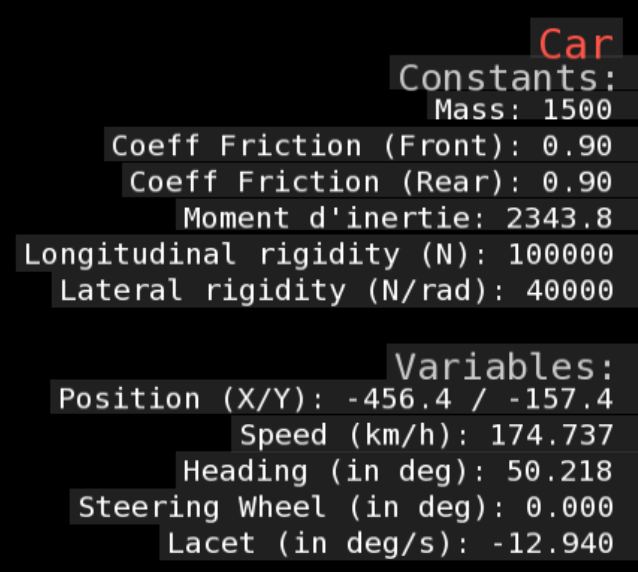
\includegraphics[width=0.5\textwidth]{resources/example_debug_mode_1}
    \caption{Exemple de mode Debug}
    \label{fig:debug_mode}
\end{figure}

\paragraph{Compteur de FPS}
La classe \texttt{FPSCounter} affiche dynamiquement le nombre d'images par seconde (\gls{fps}) dans la \texttt{\gls{hud} \glslink{view}{View}}, permettant ainsi de surveiller la fluidité de l'application.
Elle nous permet, tout au long du développement, de remarquer si une fonctionnalité que l'on vient d'implémenter est trop gourmande en ressources et de l'optimiser en conséquence.
\textsuper
Pour calculer le nombre d'images par seconde, on compte le nombre d'images générées en une seconde.
La classe contient, parmi ses attributs, un compteur d'image \texttt{frameCount}, et un accumulateur de temps \texttt{timeAccumulator}.
\begin{lstlisting}[style=CStyle, label={lst:code_fpscounter}]
void FPSCounter::update(const float dt) {
    timeAccumulator += dt;
    frameCount++;
    if (timeAccumulator >= 1.f) {
        currentFPS = frameCount;
        frameCount = 0;
        timeAccumulator = 0.f;
        text.setString("FPS: " + std::to_string(currentFPS));
    }
}
\end{lstlisting}
Le paramètre \texttt{dt} est le \gls{delta_temps} entre la dernière image et l'image actuelle.

À chaque nouvelle image et donc à chaque appel de la méthode \texttt{update()} (\S~\ref{par:class_game}) de la classe \texttt{Game}, on appelle la méthode \texttt{update()} de la classe \texttt{FPSCounter} en lui passant le \gls{delta_temps}.
On ajoute le \gls{delta_temps} à l'accumulateur de temps et on incrémente le compteur d'image.
Lorsque l'accumulateur de temps dépasse 1 seconde, on met à jour le nombre d'images par seconde et on remet le compteur d'image et l'accumulateur de temps à zéro.

\subsubsection{Affichage de la trajectoire et prédictions}\label{subsubsec:affichage-de-la-trajectoire-et-predictions}
Dans notre simulateur, la ligne de prédiction joue un rôle clé en offrant à l'utilisateur une approximation de l'évolution future du véhicule en fonction de son état et de ses entrées clavier actuelles.
Cette fonctionnalité permet de mieux comprendre l'impact immédiat des commandes de conduite, mais aussi d'anticiper les conséquences de ces actions sur le comportement global du véhicule.

\begin{figure}[H]
    \centering
    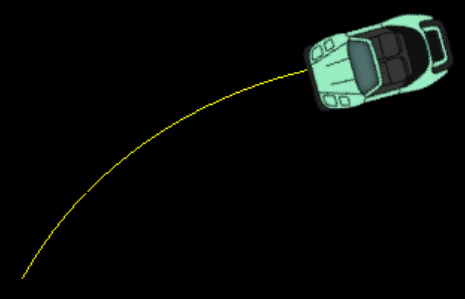
\includegraphics[width=0.5\textwidth]{resources/example_prediction_line_1}
    \caption{Exemple de ligne de prédiction des mouvements.}
    \label{fig:prediction_line}
\end{figure}

\paragraph{Calcul de la trajectoire prédictive}
Pour obtenir la trajectoire prédictive, nous simulons l'évolution du véhicule en itérant la dynamique physique sur plusieurs pas de temps à chaque image.
La méthode \texttt{computePredictionLine} procède de la manière suivante :
\begin{itemize}
    \item Le \gls{delta_temps} utilisé pour ces itérations est déterminé de manière robuste grâce à la méthode \texttt{updateAndGetMedian} (le code est définis au \S~\ref{lst:code_dequeue_dt}), qui calcule la médiane des deltas de temps récents afin de lisser les variations liées à la volatilité du temps entre images.
    \item À partir de l'état courant du véhicule, la dynamique est simulée en utilisant la méthode \texttt{getNextIterations()} de la classe \texttt{Vehicle}.
    Pour chaque itération, la nouvelle position et l'orientation sont calculées et stockées dans un tableau.
    \item Ces points, une fois convertis en coordonnées écran \textit{via} le facteur de conversion (\texttt{METER\_TO\_PIXEL} définis dans le fichier \texttt{constants.h}), représentent la trajectoire future du véhicule.
\end{itemize}

\paragraph{Tracé en temps réel \textit{via} les données issues de la simulation}
L'affichage de cette trajectoire prédictive est géré en temps réel grâce à un objet \texttt{\gls{sf_vertex_array}}\cite{sfml_sf_vertexarray} configuré en mode \texttt{LineStrip}.
À chaque frame :
\begin{itemize}
    \item Les points prédits sont recalculés et le \texttt{\gls{sf_vertex_array}} est mis à jour pour refléter le chemin futur du véhicule.
    \item La visualisation dynamique permet à l'utilisateur de voir immédiatement l'effet des commandes de conduite sur la trajectoire prévue, offrant ainsi un retour visuel direct sur l'évolution de l'état du véhicule.
    \item Cette approche interactive aide également à identifier et à ajuster les paramètres du modèle physique en observant comment de petites modifications influent sur le comportement prévisionnel.
\end{itemize}

\subsubsection{Gestion des intéractions entrée-sortie}\label{subsubsec:gestion-des-interactions-entree-sortie}
\paragraph{Événements globaux}
La gestion des interactions globale à l'application se fait \textit{via} la méthode \texttt{manageEvents()} de la classe \texttt{Game}.
Ce système s'appuie sur le mécanisme d'événements de la bibliothèque \gls{sfml}, qui capture et gère de manière asynchrone toutes les interactions (clavier, souris, redimensionnement de fenêtre, etc.)
\gls{sfml} place les événements dans une file d'attente, permettant à l'application de les traiter un par un afin d'assurer une réponse immédiate aux actions de l'utilisateur.

\begin{itemize}
    \item \textbf{Clavier} : La touche F active/désactive le compteur de \gls{fps}, F3 bascule le mode Debug, F5 réinitialise la position du véhicule et ESC ferme l'application.
    \item \textbf{Souris} : Le défilement de la molette permet d'ajuster le niveau de zoom sur la \texttt{Game \glslink{view}{View}}, offrant ainsi à l'utilisateur la possibilité de mieux suivre le véhicule ou d'obtenir une vue d'ensemble du circuit.
\end{itemize}

\paragraph{Contrôle de la voiture}
Pour ce qui est du contrôle du véhicule, les interactions sont gérées par la méthode \texttt{Car::handleInput(const float dt)}, appelé à chaque iteration de l'application.
Son but est de vérifier l'état des touches de direction (gauche, droite, haut, bas) et d'ajuster la vitesse et l'angle du véhicule en conséquence.

On peut noter qu'elle prends en paramètre le \gls{delta_temps} pour éviter un biais liés aux \gls{fps}.

Ce système d'événements, en tirant parti des fonctionnalités offertes par \gls{sfml}, assure une interactivité réactive et une expérience utilisateur intuitive.

\subsection{Optimisation du rendu et de l'affichage}\label{subsec:optimisation-du-rendu-et-de-l-affichage}
\subsubsection{Gestion des \glspl{view}}\label{subsubsec:gestion-des-vues}
Dans le simulateur, on peut distinguer deux \glspl{view} :
\begin{itemize}
    \item \textbf{\texttt{Game \glslink{view}{View}}} : C'est la \gls{view} principale où le circuit et le véhicule sont affichés.
    Elle est centrée sur le véhicule, offrant une perspective immersive de la conduite.
    \item \textbf{\texttt{\gls{hud} \glslink{view}{View}}} : Cette \gls{view} affiche des informations supplémentaires, telles que le compteur de \gls{fps} et les données de débogage (voir section~\ref{subsubsec:visualisation-des-informations-dynamiques}).
\end{itemize}

C'est ce qui nous permet de suivre le véhicule avec la \og caméra \fg{} sans que cela n'affecte les informations affichées dans la \gls{hud} \glslink{view}{View}.

\subsubsection{Optimisations mises en œuvre}\label{subsubsec:optimisations-mises-en-oeuvre}
Afin d'assurer une fluidité optimale du simulateur, plusieurs optimisations ont été mises en œuvre :
\begin{itemize}
    \item \textbf{Calcul du circuit} : Le circuit est calculé une première fois, puis stocké dans un tableau de segments de route (\texttt{\gls{std_vector}<RoadSegment>}\cite{cpp_reference_vector}).
    Lorsque le circuit a besoin d'être recalculé, par exemple lors d'une modification du zoom, un appel à la méthode \texttt{needUpdate()} de la classe \texttt{Circuit} le définit comme obsolète.
    À la prochaine itération de la boucle principale, il est recalculé et le tableau de segments de route est mis à jour.
    \item \textbf{Utilisation de Vertex Arrays} : Le tracé de la trajectoire est réalisé à l'aide d'un \texttt{\gls{sf_vertex_array}}\cite{sfml_sf_vertexarray}, ce qui permet de dessiner une série de points connectés en un seul appel de rendu.
    \item \textbf{Gestion efficace de la \gls{view}} : La \texttt{Game \glslink{view}{View}} est ajustée dynamiquement en se recentrant sur le véhicule, minimisant ainsi les recalculs inutiles et garantissant que seul le contenu pertinent est redessiné.
\end{itemize}

\subsection{Perspectives d'amélioration et évolutions futures}\label{subsec:perspectives-d-evolution}
Bien que l'interface graphique actuelle réponde aux besoins du projet, plusieurs axes d'amélioration ont été identifiés pour de futures itérations :
\begin{itemize}
    \item \textbf{Effets visuels avancés} : L'ajout d'animations, d'effets de particules ou de transitions fluides pourrait enrichir l'expérience utilisateur.
    \item \textbf{Interface utilisateur interactive} : La mise en place de menus interactifs, d'options de configuration en temps réel ou d'indicateurs graphiques plus sophistiqués permettrait de personnaliser davantage la simulation.
    \item \textbf{Optimisation \textit{via} \gls{multi_threading}} : La séparation des calculs physiques et du rendu graphique sur des threads distincts pourrait améliorer la réactivité et la fluidité du simulateur.
    \item \textbf{Extensions de la \texttt{\gls{hud} \glslink{view}{View}}} : Intégrer davantage d'informations (comme des graphiques temps réel ou des indicateurs de performance détaillés) pourrait offrir un meilleur retour utilisateur.
\end{itemize}

    \section{Bilan Technique}\label{sec:bilan-technique}

\subsection{Problèmes rencontrés et surmontés}\label{subsec:problemes-rencontres-et-surmontes}
Durant le développement du simulateur de conduite, nous avons rencontré et surmonté plusieurs difficultés, ce qui nous a permis d'approfondir nos compétences techniques et d'améliorer notre capacité à mener un bon travail en groupe.

\subsubsection{Gestion de Git}\label{subsubsec:git}
Tout au long du projet, nous avons utilisé \gls{git} et travaillé sur plusieurs \gls{git_branches} afin d'éviter les conflits de code lors du travail simultané sur les mêmes fichiers.
Malgré ces précautions, quelques conflits sont survenus lors des fusions de branches.
Avec le temps, nous avons appris à mieux gérer cette fonctionnalité de \gls{git} et à améliorer notre communication, réduisant ainsi significativement ces problèmes.

\subsubsection{Configuration avec \gls{cmake}}\label{subsubsec:cmake}
L'utilisation du fichier \texttt{CMakeLists.txt} pour gérer les bibliothèques et créer les différents exécutables a représenté un défi technique supplémentaire.
Les difficultés sont principalement survenues en raison des différences entre nos environnements de développement.
Bien que nous travaillions tous les deux sous Linux, l'un utilisait \gls{arch-linux} et l'autre \gls{ubuntu}, ce qui a engendré quelques disparités dans la gestion de certaines bibliothèques.

\subsubsection{Découverte de \gls{sfml}}\label{subsubsec:sfml}
Nous avons dû nous familiariser avec la bibliothèque \gls{sfml}, alors inconnue pour nous, et concevoir une interface graphique adaptée aux besoins du projet.
Cette phase d'apprentissage a été déterminante pour exploiter pleinement les fonctionnalités de \gls{sfml} et réaliser un rendu graphique efficace sans recourir à des techniques trop complexes.

\subsubsection{Gestion du temps et synchronisation}\label{subsubsec:la-gestion-du-temps}
La synchronisation des mises à jour, notamment la gestion du delta de temps entre les frames, a constitué un défi important.
Il a fallu ajuster nos méthodes de calcul du temps afin d’assurer une fluidité de l’animation et une réactivité optimale de l’interface.

\subsection{Retour sur les technologies utilisées}\label{subsec:retour-sur-les-technologies-utilisees}
Le choix du langage \gls{cpp} s'est révélé judicieux en raison de sa polyvalence et de ses performances.
Malgré une connaissance initiale limitée, ce projet nous a permis de progresser significativement dans sa maîtrise.
L'utilisation de \gls{sfml} a également été un atout majeur, simplifiant le développement d'interfaces graphiques interactives sans nécessiter de techniques trop complexes.
De plus \gls{gnuplot} nous a permis de pouvoir visualiser toutes les données produites par notre modèle, ce qui nous a permis de valider certaines fonctionnalités du modèle physique, et d'en corriger d'autres.

\subsection{Implémentation de la physique}\label{subsec:implem-phys}
En commançant notre projet, nous avons voulu implémenter trop de principes physiques en même temps, ce qui nous menait à de nombreuses erreurs.
Ceci nous a contraint à recommencer l'implémentation de la physique plusieurs fois.
Cette erreur nous a cependant appris qu'il ne faut pas essayer d'implémenter toutes les fonctionnalités en un bloc, mais de faire pas à pas.
C'est finalement en adoptant une manière itérative, en implémentant les différents phénomènes physique un à un, que nous avons réussi à avoir un modèle physique fonctionnel.

\subsection{Le manque de ressources}\label{subsec:manque-ressources}
L'étude de la dynamique des véhicules est quelque chose d'assez documenté, cependant aucune ressource que nous avons trouvée lie chaque phénomène physique que nous avons implémenté ensemble.
Nous avons donc dû fournir un travail de recherche approfondi pour pouvoir lier tous les phénomènes physiques entre eux.

\subsection{Le manque de données}\label{subsec:manque-data}
Similaire au manque de ressources, il y avait encore moins de données disponibles, cela voulait dire qu'après avoir implémenté les différentes formules trouvées, nous devions lancer notre modèle avec différentes données pour trouver les données qui donnaient les résultats obtenus.
De plus, cela nous a mené à plusieurs reprises, lorsqu'on implémentait une nouvelle fonctionnalité que cela casse totalement le code.
Celui-ci nous donnait alors des données dépassantes $9e^{12}$.
À chaque implémentation de nouvelles fonctionnalités, nous devions donc mener un travail de recherche pour identifier les variables qui nous posaient problème, puis en itérant notre modèle de nombreuses fois avec des données différentes, trouver les valeurs adaptées.



\subsection{Perspectives d'amélioration}\label{subsec:perspectives-d'ameliorations}
Pour une future amélioration du projet, nous avons identifié plusieurs axes d'améliorations :
\begin{itemize}
    \item Implémenter divers scénarios de conduite, afin d'offrir à l'utilisateur des expériences des différents phénomènes physiques implémentés.
    \item Comme proposé dans le sujet original, implémenter des phénomènes aléatoires, par exemple avoir un animal qui traverse la route, forçant l'utilisateur à changer sa trajectoire.
    \item Améliorer l'esthétique globale du projet, tant au niveau de l'interface graphique que des animations.
    \item Affiner le modèle physique en intégrant des phénomènes supplémentaires et en ajustant les paramètres pour une simulation encore plus réaliste.
    Plus précisément, on pourrait par exemple introduire un centre de gravité dynamique, ce qui permettrait de modéliser le transfert de forces du véhicule lors d'un freinage, d'une accélération ou de la prise d'un virage.
    \item La physique du modèle, pensée, initialement, uniquement pour l'interface graphique ne permet pas de générer une trajectoire sur un \texttt{dt} dépassant 9999.
    Bien que ce soit amplement suffisant pour l'interface, cette limite restraint la visualisation d'un scénario fixe en traçant les graphiques des différentes données.
    \item Pour une meilleure expérience utilisateur, nous pourrions également ajouter un moteur audio à notre simulateur.

\end{itemize}

\subsection{Ce que nous ferions différemment}\label{subsec:ce-que-nous-ferions-differemment}
Avec le recul, nous aurions intégré dès le départ des tests unitaires et d'intégration afin de détecter plus rapidement les erreurs et d'améliorer la robustesse du code.
Une phase de planification et de prototypage plus approfondie aurait permis de réduire les imprévus liés à l'apprentissage de nouvelles bibliothèques, notamment \gls{sfml}\@.
Ce changement méthodologique aurait sans doute accéléré le développement et renforcé la qualité du produit final.

\subsection{Mise en route du projet}\label{subsec:mise-en-route-du-projet}

\subsubsection{Dépendances}\label{subsubsec:dependances}
Pour compiler le projet, il est nécessaire d'installer les dépendances suivantes :
\begin{itemize}
    \item \textbf{Un compilateur supportant \gls{cpp}17} : par exemple, \texttt{clang++} ou \texttt{g++}.
    \item \texttt{\gls{cmake}} (version 3.30 ou supérieure) : pour la configuration et la gestion de la compilation.
    \item \texttt{\gls{sfml}} (versions $\left[2.5 ; 3.0\left[$) : pour la gestion de l'interface graphique et des entrées.
    \item \texttt{\gls{gnuplot}} : pour la génération des graphiques.
    \item \texttt{\gls{boost}} : utilisé pour la manipulation des flux, particulièrement en lien avec \texttt{\glspl{gnuplot}}.
    \item \texttt{\gls{googletest}} : installé automatiquement via le fichier \texttt{CMakeLists.txt}, pour la réalisation des tests unitaires.
\end{itemize}
\newpage
\subsubsection{Installation}\label{subsubsec:installation}
Le projet est disponible sur \gls{github} à l'adresse suivante : \url{https://github.com/QuentinRdl/Driving-Sim/}.

Pour l'installer, il est nécessaire de cloner le dépôt et de construire les exécutables correspondants aux différentes parties du projet grâce à ces commandes :

\begin{lstlisting}[style=bashStyle,label={lst:build}]
git clone 'https://github.com/QuentinRdl/Driving-Sim.git' && cd Driving-Sim
mkdir -p build && cd build
cmake ..
make
\end{lstlisting}
\noindent
Expliquons brièvement ces commandes :
\begin{itemize}
    \item La 1\textsuperscript{ère} ligne (\texttt{git clone}\dots) clone le dépôt et se rend dans le dossier cloné.
    \item La 3\textsuperscript{ème} ligne (\texttt{mkdir}\dots) crée un dossier \texttt{build} dans lequel on va construire les exécutables et s'y déplacer.
    \item Les lignes 4 (\texttt{cmake ..}) et 5 (\texttt{make}) permettent de configurer le projet et de compiler les exécutables.
\end{itemize}

\noindent
Une fois fait, il est possible de lancer les différents exécutables :
\begin{itemize}
    \item \texttt{Driving\_Sim} : pour le simulateur de conduite.
    \item \texttt{DrivingSim\_test} : pour les tests unitaires.
    \item \texttt{DrivingSim\_plot} : pour la génération des graphiques.
\end{itemize}


%    \glsaddall
    \printglossaries
    \newpage

    \begin{thebibliography}{9}
        \bibitem{euler_explicite}
        Frédéric Legrand.
        Intégration des équations différentielles : méthode d'Euler.
        Disponible à l'adresse : \url{https://www.f-legrand.fr/scidoc/srcdoc/numerique/euler/eulers/eulers-pdf.pdf}.

        \bibitem{slip-angle}
        Your Data Driven.
        Tyre Slip Angle – 2 Clear Explanations.
        Disponible à l'adresse : \url{https://www.yourdatadriven.com/tyre-slip-angle-explained}.

        \bibitem{vtech}
        Virginia Tech University.
        Chapter 2, Vehicle Dynamics Modeling.
        Disponible à l'adresse : \url{https://vtechworks.lib.vt.edu/server/api/core/bitstreams/fe6d4ca1-514b-4e2b-b1ac-6561824a9de1/content}.
        Sous licence \textit{Creative Commons Attribution 4.0 International}.

        \bibitem{VDS_MathWorks}
        MathWorks.
        Modeling a Vehicle Dynamics System.
        \url{https://www.mathworks.com/help/ident/ug/modeling-a-vehicle-dynamics-system.html}

        \bibitem{fermi2023}
        Thomas Fermi.
        Kinematic Bicycle Model.
        Disponible à l'adresse : \url{https://thomasfermi.github.io/Algorithms-for-Automated-Driving/Control/BicycleModel.html#kinematic-bicycle-model}.
        Sous licence \textit{Creative Commons Attribution 4.0 International}.

        \bibitem{RK4}
        Swarthmore College.
        Fourth Order Runge-Kutta.
        Disponible sur : \url{https://lpsa.swarthmore.edu/NumInt/NumIntFourth.html}

        \bibitem{cpp_reference_push_back}
        Contributeurs de cppreference.com. \\
        ``\texttt{std::\gls{deque}::push\_back} - Référence \gls{cpp}''. \\
        Disponible sur : \url{https://en.cppreference.com/w/cpp/container/deque/push_back}.

        \bibitem{cpp_reference_pop_front}
        Contributeurs de cppreference.com.\\
        ``\texttt{std::\gls{deque}::pop\_front} - Référence \gls{cpp}''.\\
        Disponible sur : \url{https://en.cppreference.com/w/cpp/container/deque/pop_front}.

        \bibitem{cpp_reference_vector}
        Contributeurs de cppreference.com.\\
        ``\texttt{\gls{std_vector}} - Référence \gls{cpp}''.\\
        Disponible sur : \url{https://en.cppreference.com/w/cpp/container/vector/vector}.

        \bibitem{cpp_reference_std_nth_element}
        Contributeurs de cppreference.com.\\
        ``\texttt{\gls{std_nth_element}} - Référence \gls{cpp}''.\\
        Disponible sur : \url{https://en.cppreference.com/w/cpp/algorithm/nth_element}.

        \bibitem{cpp_reference_std_sort}
        Contributeurs de cppreference.com.\\
        ``\texttt{\gls{std_sort}} - Référence \gls{cpp}''.\\
        Disponible sur : \url{https://en.cppreference.com/w/cpp/algorithm/sort}.

        \bibitem{cpp_reference_std_unordered_map}
        Contributeurs de cppreference.com.\\
        ``\texttt{\gls{std_unordered_map}} - Référence \gls{cpp}''.\\
        Disponible sur : \url{https://en.cppreference.com/w/cpp/container/unordered_map}.

        \bibitem{cpp_reference_std_unique_ptr}
        Contributeurs de cppreference.com.\\
        ``\texttt{\gls{std_unique_ptr}} - Référence \gls{cpp}''.\\
        Disponible sur : \url{https://en.cppreference.com/w/cpp/container/unordered_map}.

        \bibitem{documentationSFML}
        Documentation de la \gls{sfml}. \\
        Disponible sur : \url{https://www.sfml-dev.org/documentation/}.

        \bibitem{sfml_sf_texture}
        Contributeurs de sfml-dev.org.\\
        ``\texttt{sf::Texture} - \gls{sfml} Documentation''.\\
        Disponible sur : \url{https://www.sfml-dev.org/documentation/3.0.0/classsf_1_1Texture.html}

        \bibitem{sfml_sf_vertexarray}
        Contributeurs de sfml-dev.org.\\
        ``\texttt{\gls{sf_vertex_array}} - \gls{sfml} Documentation''.\\
        Disponible sur : \url{https://www.sfml-dev.org/documentation/3.0.0/classsf_1_1VertexArray.html}

        \bibitem{stackoverflow_embed_font}
        Karol Szustakowski (2017).
        \gls{stackoverflow} \\
        Disponible sur : \url{https://stackoverflow.com/a/45802538}
    \end{thebibliography}

    \clearpage
    \vspace*{\fill}
    \begin{center}
    {\Large \textbf{Résumé}}
    \end{center}
    \bigskip
    \noindent
    \begin{minipage}{\textwidth}
        Ce rapport présente le développement d'un prototype d'un simulateur de conduite réalisé en \gls{cpp}.
        L'objectif principal est de modéliser de manière réaliste divers scénarios de conduite en développant un modèle de physique réaliste pour avoir une gestion dynamique du véhicule par l'utilisateur.
        L'architecture modulaire et orienté objet du code source est pensée pour faciliter l'ajout de nouvelles fonctionnalités.

        \bigskip

        This report presents the development of a prototype for a driving simulator realized in \gls{cpp}.
        The main objective is to realistically model multiple driving scenarios using a realistic vehicle dynamics model so that the user can dynamically manage the vehicle.
        The source code uses a modular architecture and is object-oriented to facilitate adding new features.
    \end{minipage}
    \vspace*{\fill} % Espace après pour centrer verticalement
    \clearpage
\end{document}